\documentclass{beamer}

\mode<presentation>
{
  \usetheme{CambridgeUS}      % or try Darmstadt, Madrid, Warsaw, ...
  \usecolortheme{default} % or try albatross, beaver, crane, ...
  \usefonttheme{default}  % or try serif, structurebold, ...
  \setbeamertemplate{navigation symbols}{}
  \setbeamertemplate{caption}[numbered]
  \setbeamertemplate{bibliography item}[text]
} 

\usepackage[english]{babel}
\usepackage[utf8x]{inputenc}
\usepackage[document]{ragged2e}
\usepackage{amsmath}

\usepackage{listings}
\usepackage{color}

\lstset{frame=tb,
  breaklines=true,
  postbreak=\mbox{\textcolor{red}{$\hookrightarrow$}\space},
  basicstyle=\ttfamily,
  keywordstyle=\color{blue}\ttfamily,
  stringstyle=\color{red}\ttfamily,
  commentstyle=\color{green}\ttfamily,
  morecomment=[l][\color{magenta}]{\#}
}

\title[Applied Parallel Programming]{Bilinear Interpolation Upsampling on CUDA}
\subtitle{Project Phase-I}
\author{Bilgin AKSOY}

\institute{\bf Informatics Enstitute}
\logo{
\includegraphics[scale=0.2]{./Figures/iilogo.png}}
\date{13 Nov 2017}

\begin{document}

	\begin{frame}
	  \titlepage
	\end{frame}

% Problem definitons
\section{Introduction}

	\begin{frame}{Problem}
		
		\begin{itemize}
		  \item A deep network for object segmentation.  
		  \item \justifying This network has 5 two-by-two max-pooling layer, each of which downsamples its input by factor two. 
		\end{itemize}
		\begin{figure}
		  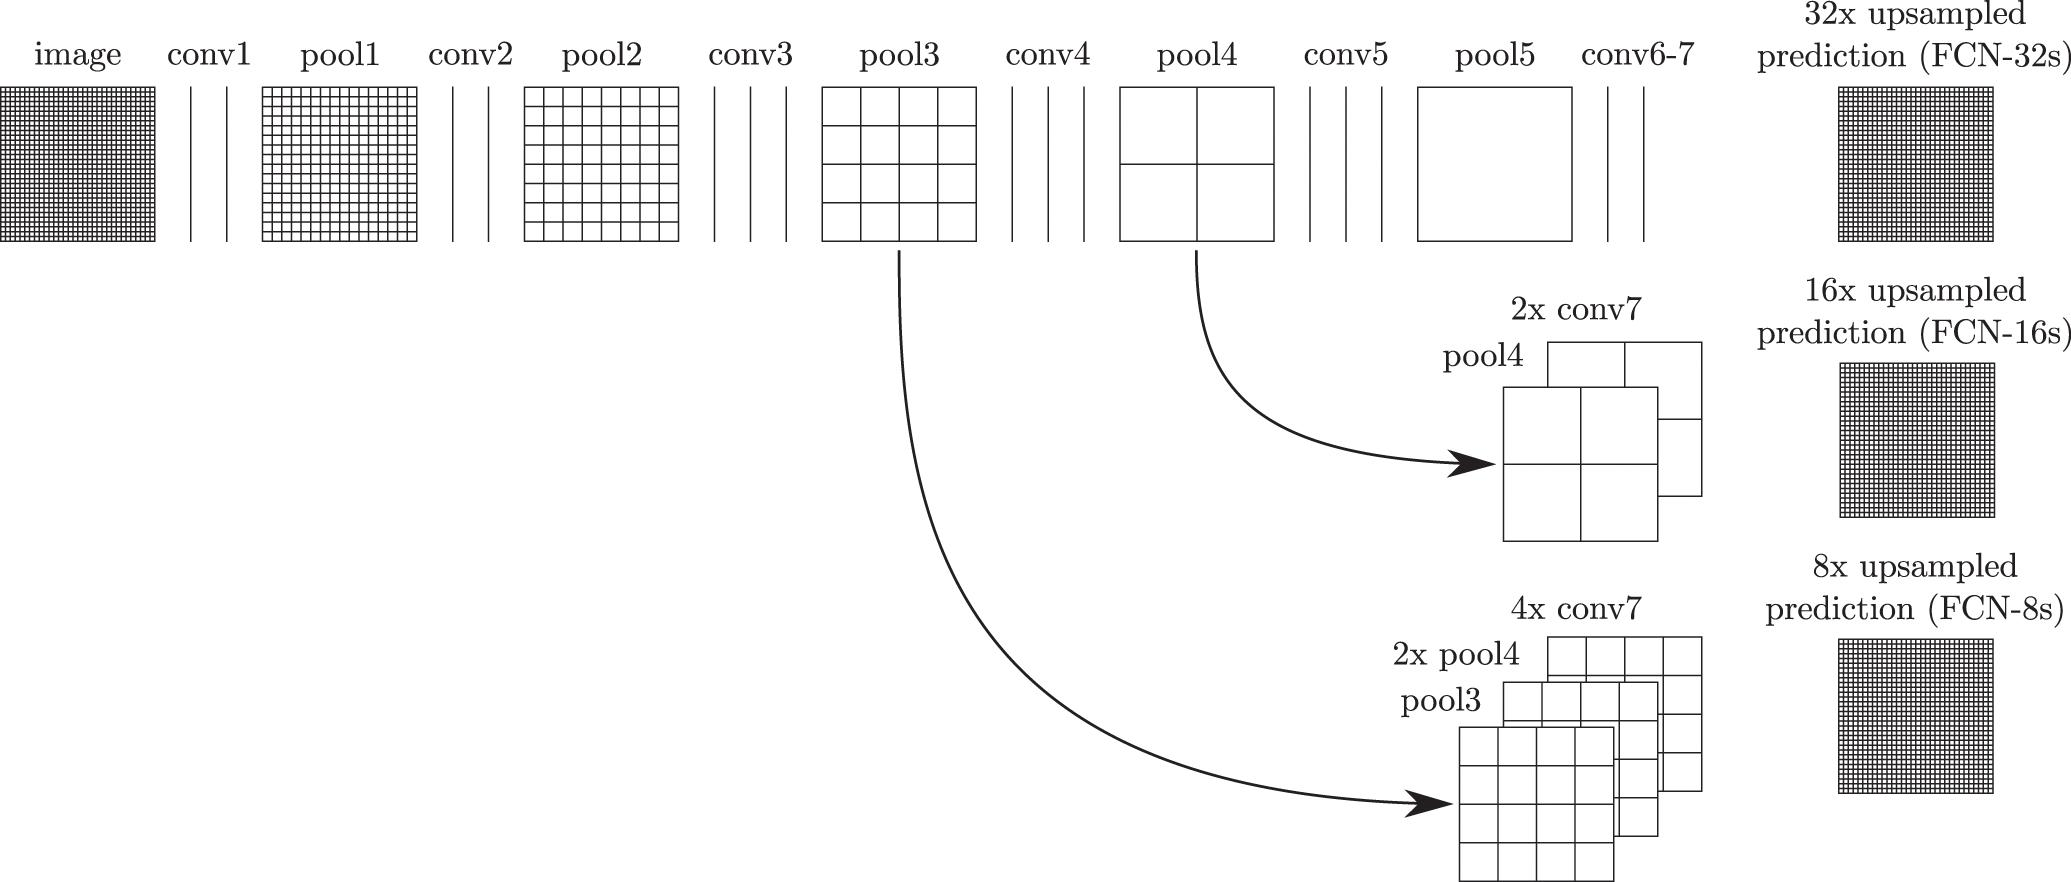
\includegraphics[scale=0.15]{./Figures/DAGnet.jpg}
		  \caption{\label{fig:DAGnet}Network Architecture-Long et al.\cite{long2015fully}}
		\end{figure}	
	\end{frame}
	%next slide
	\begin{frame}{Problem (cont'd)}
		\begin{itemize}
				\item After pool3, the activation size have been reduced by factor $8= 2^3 $.
				\item After pool4, the activation size have been reduced by factor $16= 2^4 $.
				\item After pool5, the activation size have been reduced by factor $32= 2^5 $.
		\end{itemize}
		\begin{figure}
					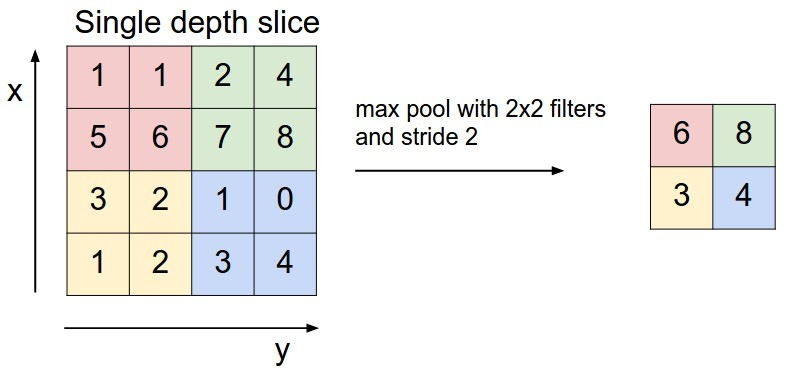
\includegraphics[scale=0.3]{./Figures/maxpool.jpeg}
					\caption{Max-Pooling - Image from \url{http://cs231n.github.io/convolutional-networks}}
		\end{figure}
	\end{frame}
	%next slide
	\begin{frame}{Problem (cont'd)}
		\begin{itemize}
			\item \justifying At the end of the final layer, sum three activations and calculate the error(loss) and back-propagate the error to be able to minimize the error.
		\end{itemize}
		\begin{figure}
			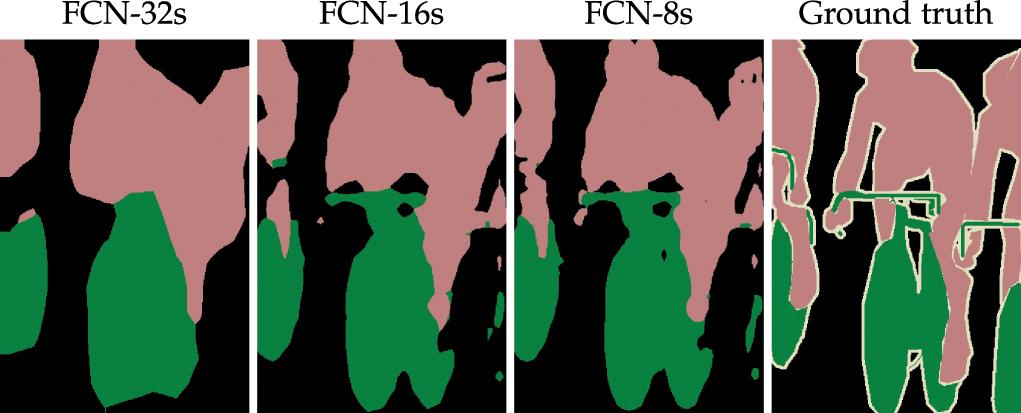
\includegraphics[scale=0.15]{./Figures/fcn_output.jpg}
			\caption{\label{fig:fcn_output}Activations of Pooling Layers-Long et al.\cite{long2015fully}}
		\end{figure}
	\end{frame}
	%next slide
	\begin{frame}{Problem (cont'd)}
		\begin{itemize}
			\item\justifying I will implement a bilinear interpolation upsampling kernel and my kernel will not only upsample the activations but also produce the final result by summing the activations.
			\item\justifying This kernel should also work on Python environment (by using Cython / PyCUDA).
		\end{itemize}
	\end{frame}
	
%Literature Survey	
\section{Literature}
	%next slide
	\begin{frame}{Literature Survey}
		\begin{itemize}
			\item \justifying \textbf{\underline{Bilinear Interpolation:}} Bilinear interpolation is used to know values at 	random position from the weighted average of the 	four closest pixels to the specified input coordinates, and assigns that value to the output coordinates.\cite{fadnavis2014image}  \eqref{equ:bilinear}
		\end{itemize}
	\end{frame}
	%next slide
	\begin{frame}{Literature Survey (cont'd)}
		\begin{figure}
			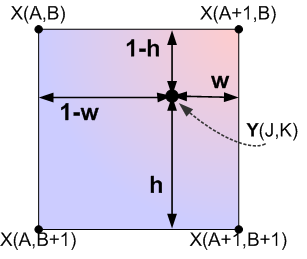
\includegraphics[scale=0.5]{./Figures/bilinear_interpolation.png}
			\caption{\label{fig:bilinear_img}Image from \url{https://www.giassa.net/?page_id=240}\cite{bilinear_img}}
		\end{figure}
		\begin{multline}\label{equ:bilinear}
			Y(J,K)=(1-W)(1-H)X(A,B)+(W)(1-H)X(A+1,B)+\\(1-W)(H)X(A,B+1)+(W)(H)X(A+1,B+1)
		\end{multline}\vskip 4 cm
	\end{frame}
	%next slide
	\begin{frame}{Literature Survey (cont'd)}
		\begin{itemize}
			\item\justifying Qingshuang et al.\cite{qingshuang2013parallel} proposed "GPGPU-based parallel algorithm can take full advantage of the GPU's parallel computing capabilities, and can achieve about 40 times speedup."
		\end{itemize}
		%table-1
		\begin{table}[H] % H stands for here not anywhere else
			\centering	
			\caption[The Time-Consuming Of Serial And Parallel Bilinear Spatial Interpolation Of Different Grid Size]{\justifying The Time-Consuming Of Serial And Parallel Bilinear Spatial Interpolation Of Different Grid Size \cite{qingshuang2013parallel}}
			\label{tab:table_1}
			\begin{tabular}{l c c }
				Grid Size & CPU (sec) & GPU (sec)\\ \hline\hline 
				40x40 & 1.70 & 0.11 \\  \hline
				100x100 & 10.34 & 0.37 \\ \hline
				200x200 & 41.43 & 1.21 \\ \hline
				300x300 & 93.13 & 2.36 \\ \hline
				500x500 & 240.02 & 5.70 \\ \hline
				800x800 & 630.92 & 14.40 \\ \hline
				1200x1200 & 1432.33 &  32.41 \\ \hline
			\end{tabular}
		\end{table}
	\end{frame}
	%Next slide
	\begin{frame}
		\begin{itemize}
			\item\justifying Akgün and Gevrekci have been proposed "a massively multi-threaded implementation of super-resolution image formation on the NVIDIA CUDA architecture." \cite{akgun2013accelerating} "Super-resolution reconstruction begins with an initial estimate image which is typically chosen as a bilinearly upscaled version of the original low resolution frame."
		\end{itemize}
		%table-2
		\begin{table}[H] % H stands for here not anywhere else
			\centering	
			\caption[Bilinear filtering code analysis]{Bilinear filtering code analysis \cite{akgun2013accelerating}}
			\label{tab:table_2}
			\begin{tabular}{l c}
			    \hline\hline
				Thread numbers (x,y) &(32,32) \\ \hline 
				Shared memory bank conflict & N/A \\ \hline
				Global memory BW efficiency & 100 \\ \hline
				Register usage & 17 \\ \hline
				Occupancy & 0,877 \\ \hline
				Total execution time per frame & 161 microsec\\ \hline
			\end{tabular}
		\end{table}
	\end{frame}
	%Next slide
	\begin{frame}[fragile]{Literature Survey (cont'd)(Real Life Examples)}
		\begin{block}{OpenCV CPU}		
			\begin{lstlisting}[language=C]
			void 	cv::resize (
			InputArray src, OutputArray dst, Size dsize, double fx=0, double fy=0, int interpolation=INTER_LINEAR
			)
			\end{lstlisting}
		\end{block}
		\begin{block}{OpenCV GPU}		
		
			\begin{lstlisting}[language=C]
			void cv::cuda::resize	(
			InputArray src, OutputArray dst, Size dsize, double fx = 0, double fy = 0, int interpolation = INTER_LINEAR, Stream &stream=Stream::Null() 
			)	
			\end{lstlisting}
		\end{block}
	\end{frame}
	%Next slide
	\begin{frame}[fragile]{Literature Survey (cont'd)(Real Life Examples)}
		\begin{block}{Intel Integrated Performance Primitives(CPU Optimizations)}
			\begin{lstlisting}[language=C]
				IppStatus ippiResizeLinear_<mod>(const Ipp<datatype>* pSrc, Ipp32s srcStep, Ipp<datatype>* pDst, Ipp32s dstStep, IppiPoint dstOffset, IppiSize dstSize, IppiBorderType border, const Ipp<datatype>* pBorderValue, const IppiResizeSpec_32f* pSpec, Ipp8u* pBuffer)
			\end{lstlisting}
		\end{block}
		\begin{itemize}
			\item Just for Intel CPU. Not free.(249\$for Academic Licence)
			\item\justifying OpenCV 3.x has native support for IPP-ICV library which is a special subset of Intel IPP functions for image processing and computer vision.
		\end{itemize}
	\end{frame}
	%Next slide
	\begin{frame}[fragile]{Literature Survey (cont'd)(Real Life Examples)}
		\begin{block}{Linux Command Line Tool - Imagemagick (CPU Only, OpenCL For Some Algorithms-No information avout Bilinear Upsampling)}
			\begin{lstlisting}[language=bash]
				$ convert input.jpg -scale 200% -interpolate bilinear output.jpg
			\end{lstlisting}
		\end{block}
	\end{frame}

	
%References
\section{References}
	%next slide
	\begin{block}{References}
	\end{block}
	\bibliography{./References/ref.bib}
	\bibliographystyle{ieeetr}

\end{document}